\section{Auswertung}
\label{sec:auswertung}
In den folgenden Unterabschnitten werden die verschiedenen Messungen dargestellt und ausgewertet.

\FloatBarrier %TODO: Das muss schöner gehen :)
\subsection{Reflexionsgesetz}
\label{sec:auswertung:reflexionsgesetz}
Zur Verifizierung des Reflexionsgesetzes werden
für verschiedene Einfallswinkel $\alpha_1$ die Ausfallswinkel $\alpha_2$ gemessen,
wie \autoref{tab:mess_reflexionsgesetz} zeigt.

\begin{table}
    \centering
    \caption{Messwerte zum Reflexionsgesetz.}
    \label{tab:mess_reflexionsgesetz}
    \begin{tabular}{S S}
        \toprule
        {$\alpha_1 \mathbin{/} \si{\degree}$} &
        {$\alpha_2 \mathbin{/} \si{\degree}$} \\
        \midrule
        \expandableinput{build/tab/mess_reflexionsgesetz.tex}
        \bottomrule
    \end{tabular}
\end{table}

Nach dem Reflexionsgesetz \eqref{eqn:reflexionsgesetz} ist anzunehmen,
dass der Einfallswinkel dem Ausfallswinkel genau entspricht.
Daher wird die mittlere Abweichung $\overline{|\alpha_1 - \alpha_2|}$ bestimmt.
Sie beträgt $\SI{1.357}{\degree}$.

Im Rahmen der Messgenauigkeit,
für die hier jedoch ein empirischer Wert fehlt,
stimmen Einfallswinkel und Ausfallswinkel also überein.
Damit ist das Reflexionsgesetz verifiziert.


Eine alternative Betrachtungsweise ist das Ausführen einer Regressionsrechnung.
Die bestimmten Parameter der Regressionsgerade $\alpha_2 = a \alpha_1 + b$ lauten
$a = \num{0.982(9)}$ und $b = \SI{1.89(28)}{\degree}$.
\autoref{fig:plt_reflexionsgesetz} zeigt die Messwerte und die daraus bestimmte Regressionsgerade
sowie die ideale Gerade $\alpha_1 = \alpha_2$ beziehungsweise $a=1, b=0$.

\begin{figure}
    \centering
    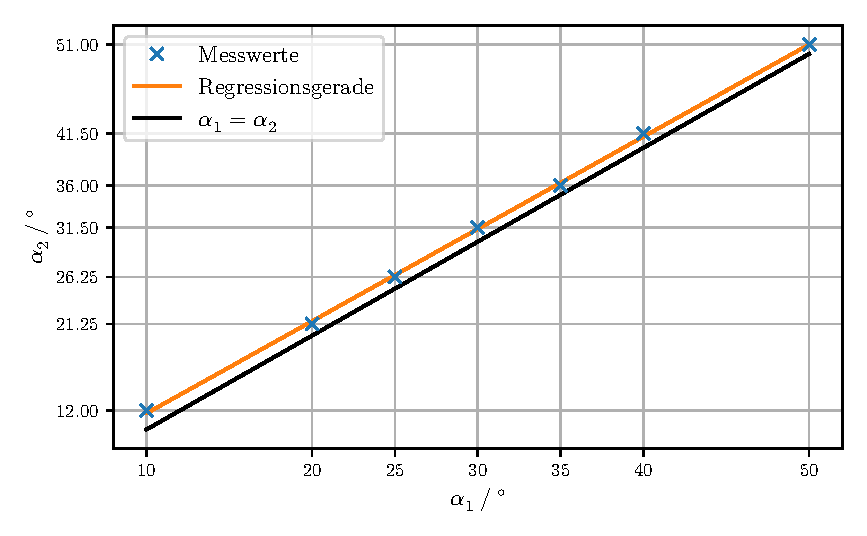
\includegraphics[width=\textwidth]{build/plt/reflexionsgesetz.pdf}
    \caption{Einfallswinkel in Abhängigkeit des Ausfallswinkels.}
    \label{fig:plt_reflexionsgesetz}
\end{figure}


\FloatBarrier %TODO: Das muss schöner gehen :)
\subsection{Brechungsgesetz}
\label{sec:auswertung:brechungsgesetz}
\autoref{tab:mess_brechungsgesetz} zeigt die
an der
\hyperref[sec:durchfuehrung:brechung:planparallele_platte]{planparallelen Platte}
aufgenommenen Messwerte zum Brechungsgesetz.
% welche aus … hervorgingen.
Dabei ist $\alpha$ der Einfallswinkel und $\beta$ der Brechungswinkel.

\begin{table}
  \centering
  \caption{Messwerte zum Brechungsgesetz.}
  \label{tab:mess_brechungsgesetz}
  \begin{tabular}{S S}
    \toprule
    {$\alpha \mathbin{/} \si{\degree}$} &
    {$\beta \mathbin{/} \si{\degree}$} \\
    \midrule
    \expandableinput{build/tab/mess_brechungsgesetz.tex}
    \bottomrule
  \end{tabular}
\end{table}

Nach Einsetzen von $n_1 \approx 1$ für Luft als erstes Medium
in das Snellius'schen Brechungsgesetz \eqref{eqn:brechungsgesetz}
kann der Brechungsindex des zweiten Mediums direkt als
\[ n_2 = n = \frac{\sin\alpha}{\sin\beta} \]
bestimmt werden.
Im Mittel ergibt sich $n = \num{1.45(2)}$.

Die Lichtgeschwindigkeit $v$ in Plexiglas kann ebenfalls
aus dem Brechungsgesetz \eqref{eqn:brechungsgesetz} gewonnen werden:
% \begin{align*}
%   \frac{v_1}{v_2} &= \frac{n_2}{n_1}
%   \tag{$v_1 =: c; n_1 =: 1; v_2 =: v; n_2 =: n$} \\
%   \Rightarrow
%   \frac{c}{v_2} &= n \\
%   \Leftrightarrow
%   v_2 &= \frac{c}{n} \ . \\
% \end{align*}
% \begin{align*}
%   \frac{v_1}{v_2} &= \frac{\sin\alpha}{\sin\beta}
%   \tag{$v_1 =: c; v_2 =: v$} \\
%   \Rightarrow
%   % \frac{c}{v} &= \frac{\sin\alpha}{\sin\beta} \\
%   % \Leftrightarrow
%   % \frac{v}{c} &= \frac{\sin\beta}{\sin\alpha} \ .
%   % \Leftrightarrow
%   v &= c \frac{\sin\beta}{\sin\alpha} \ .
% \end{align*}
\begin{align*}
  \frac{v_1}{v_2} &= \frac{\sin\alpha}{\sin\beta}
  \tag{$v_1 =: c; v_2 =: v$} \\
  \Rightarrow
  v &= c \frac{\sin\beta}{\sin\alpha}
  = \frac{c}{n} \ .
\end{align*}

Im Mittel ergibt sich $v = \SI{2.068(26)e8}{\meter\per\second}$.


\FloatBarrier %TODO: Das muss schöner gehen :)
\subsection{Strahlversatz}
\label{sec:auswertung:strahlversatz}
Für den Strahlversatz bei einer planparallelen Platte
wurden keine Messwerte aufgenommen.
Allerdings kann dieser für gegebene Einfallswinkel $\alpha$
aus \eqref{eqn:strahlversatz} berechnet werden.
Als Brechungsindex wird der
in \autoref{sec:auswertung:brechungsgesetz} bestimmte Wert $n = \num{1.45}$ angenommen;
die Länge der Platte entlang des Lots ist mit $d = \SI{5.85}{\centi\meter}$ gegeben.

In \autoref{tab:strahlversatz} sind beispielhaft Werte
für den Winkelbereich $\SI{0}{\degree} \leq \alpha \leq \SI{90}{\degree}$
angegeben;
\autoref{fig:plt_strahlversatz} stellt den Zusammenhang grafisch dar.

\begin{figure}
    \centering
    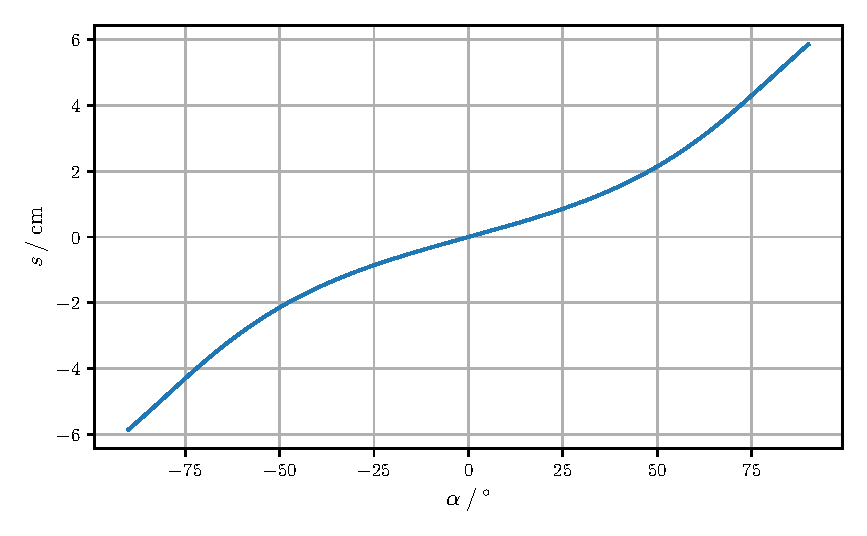
\includegraphics[width=\textwidth]{build/plt/strahlversatz.pdf}
    \caption{Strahlversatz in Abhängigkeit des Winkels.}
    \label{fig:plt_strahlversatz}
\end{figure}

\begin{table}
  \centering
  \caption{Berechneter Strahlversatz in Abhängigkeit des Einfallswinkels.}
  \label{tab:strahlversatz}
  \begin{tabular}{S S}
    \toprule
    {$\alpha \mathbin{/} \si{\degree}$} &
    {$s \mathbin{/} \si{\centi\meter}$} \\
    \midrule
    \expandableinput{build/tab/strahlversatz.tex}
    \bottomrule
  \end{tabular}
\end{table}


\FloatBarrier %TODO: Das muss schöner gehen :)
\subsection{Prisma}
\label{sec:auswertung:prisma}
Für diese Messreihe wurden in Abhängigkeit vom Einfallswinkel $\alpha_1$
die Ausfallswinkel
$\alpha_{2, \text{grün}}$ für den grünen Laser
beziehungsweise
$\alpha_{2, \text{rot}}$ für den roten Laser
bestimmt.

Es soll nun die Ablenkung $\delta$ bestimmt werden,
wie sie in \autoref{fig:prisma} dargestellt war.
%
% NOTE: Die Abhängigkeit von der Wellenlänge, die die Versuchsanleitung extra betont,
% ist bei den verwendeten Formeln implizit durch die Lichtgeschwindigkeit
% und somit die Brechungszahl gegeben.
%
Die Formel \eqref{eqn:ablenkung} für die Ablenkung $\delta$
benötigt neben den gemessenen Werten
für Einfallswinkel $\alpha_1$ und Austrittswinkel $\alpha_2$
auch die Brechungswinkel $\beta_1$ und $\beta_2$.
Wegen der Winkelbeziehung $\beta_1 + \beta_2 = \gamma$
kann jedoch auch der brechende Winkel
$\gamma = \SI{60}{\degree}$ \cite{versuchsanleitung}
des benutzten Prismas eingesetzt werden.
Der Brechungsindex für Kronglas beträgt $n = \num{1.510}$ \cite{n_kronglas}.

Die so gewonnenen Ablenkungen $\delta$ sind zusammen mit den Messwerten in \autoref{tab:prisma} aufgelistet.

\begin{table}
  \centering
  \caption{Am Prisma gemessene Einfallswinkel, Austrittswinkel und die daraus berechnete Ablenkung.} % Außerdem die Differenz der Ablenkung…
  \label{tab:prisma}
  \begin{tabular}{S S S S S S}
    \toprule
    {$\alpha_1 \mathbin{/} \si{\degree}$} &
    {$\alpha_{2, \text{grün}} \mathbin{/} \si{\degree}$} &
    {$\delta_\text{grün} \mathbin{/} \si{\degree}$} &
    {$\alpha_{2, \text{rot}} \mathbin{/} \si{\degree}$} &
    {$\delta_\text{rot} \mathbin{/} \si{\degree}$} &
    {$(\delta_\text{grün} - \delta_\text{rot}) \mathbin{/} \si{\degree}$} \\
    \midrule
    \expandableinput{build/tab/prisma.tex}
    \bottomrule
  \end{tabular}
\end{table}


\FloatBarrier %TODO: Das muss schöner gehen :)
\subsection{Beugung am Gitter}
\label{sec:auswertung:beugung}
Wie in \autoref{sec:durchfuehrung:beugung} beschrieben,
wurden für Gitter unterschiedlicher Gitterkonstanten $d$
und zugleich mit zwei Lasern der Wellenlängen
$\lambda = \SI{635}{\nano\meter}$ (rot) und
$\lambda = \SI{532}{\nano\meter}$ (grün)
die zu den Intensitätsmaxima gehörigen Ablenkwinkel gemessen.
Zusammen mit der Beugungsordnung $k$ sind die gewonnenen Messwerte
in \autoref{tab:mess_beugung} aufgeführt.

\begin{table}
  \centering
  \caption{Messwerte zur Beugung am Gitter.}
  \label{tab:mess_beugung}
  \begin{tabular}{S S S S S S S}
    \toprule
    &
    \multicolumn{2}{c}{$d = \SI{100}{\per\milli\meter}$} &
    \multicolumn{2}{c}{$d = \SI{200}{\per\milli\meter}$} &
    \multicolumn{2}{c}{$d = \SI{600}{\per\milli\meter}$} \\
    \cmidrule(lr){2-3}
    \cmidrule(lr){4-5}
    \cmidrule(lr){6-7}
    {$k$} &
    {grün} &
    {rot} &
    {grün} &
    {rot} &
    {grün} &
    {rot} \\
    \midrule
    \expandableinput{build/tab/mess_beugung.tex}
    \bottomrule
  \end{tabular}
\end{table}

Die \autoref{fig:mess_beugung} visualisiert die gemessenen Ablenkwinkel.
Es sei angemerkt,
dass die Intensitätsmaxima tatsächlich punktförmig sind;
es wurden nur zur besseren Erkennbarkeit Linien verwendet.
Sich überschneidende rote und grüne Linien werden dunkelgrün dargestellt.

\begin{figure}
    \centering
    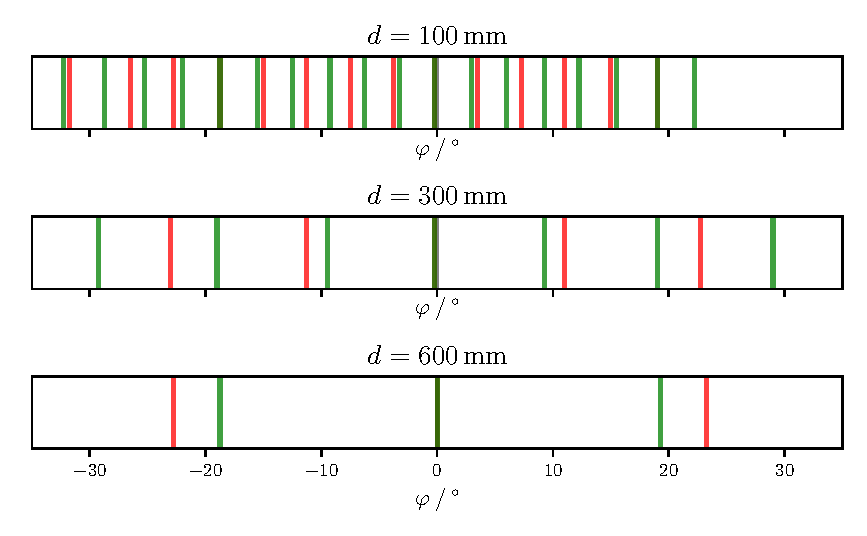
\includegraphics[width=\textwidth]{build/plt/beugung.pdf}
    \caption{Intensitätsmaxima in Abhängigkeit des Ablenkwinkels für verschiedene $d$ und $\lambda$.}
    \label{fig:mess_beugung}
\end{figure}

Nach Umstellen von \eqref{eqn:intensitaetsmaxima} kann
für jedes Intensitätsmaximum der Ordnung $k \neq 0$
die zugehörige Wellenlänge berechnet werden:

\begin{align*}
  k \lambda &= d \cdot \sin\alpha \\
  \Leftrightarrow
  \lambda &= \frac{d \cdot \sin\alpha}{k}  \ .
\end{align*}

Wird die Wellenlänge für jedes Intensitätsmaximum bestimmt
und anschließend ein Mittelwert gebildet,
ergibt sich
$\lambda = \SI{538.52(177)}{\nano\meter}$ für den grünen und
$\lambda = \SI{644.60(242)}{\nano\meter}$ für den roten Laser.
